\chapter{Testing}
\label{7-test}

To test the application I used Cucumber with user stories for acceptance tests with Zombie as a headless browser and Istanbul for code coverage testing. I also used a mock server to get mock data during testing, because the back end modules are not finished yet.

Due the simpleness of the implemented methods, e.g., getters to provide data from the model through the controller to the view, or setters to store the downloaded data in the model, I did not create unit tests.

\section{Testing}
\subsection{Acceptance Tests}
An acceptance test validates that this is the software or feature the customer wanted. I wrote user stories \see{spec-user-story} for the features I wanted to test based on the user stories I wrote during the specification phase~\cite{szofttech}.

\subsubsection{Cucumber}
\label{cucumber-test}

I used Cucumber \see{spec-cucumber} to implement acceptance tests. I used the instructions on the Cucumber website to start the implementation~\cite{github-cucumberjs}. A Cucumber test requires the following files:

\begin{itemize}
	\item \textbf{Features Files:} The user stories are stored in feature files.
	\item \textbf{Support Files:} These will be run before each scenario to create the test environment. In my case it creates a headless browser. One example is included on the Cucumber website, but that does not work. I implemented my own support file.
	\item \textbf{Step Definitions:} These are the implemented feature steps. I generated the functions with a JetBrains plugin~\cite{jetbrains-cucumber} and implemented the logic for every step. 
\end{itemize}

\subsubsection{Zombie}
I wanted to use a browser to test the client's JavaScript code. My first choice was Selenium~\cite{selenium} with a Google Chrome browser, but the tests were slow. To solve this issue I have decided to use a browser without a user interface. I chose Zombie, because it was recommended on the Cucumber website.

Zombie~\cite{zombie} is lightweight framework, that implements a browser without a user interface. It also supports assertions, that makes it possible to text field comparison and HTML element existence testing easier, and pipelines to log the outgoing requests from the Zombie browser. 

\subsection{Code Coverage Tests}
A coverage test measures which functions, statements, lines were executed~\cite{szofttech}. I tested which user story step definitions were executed, and how many times were they executed, because some scenarios had similar steps, e.g., the 8 different of filling the password fields on the settings page.

\subsubsection{Istanbul}
Istanbul~\cite{istanbul} is a code coverage software tool for JavaScript. It checks coverage for:

\begin{itemize}
	\item \emph{Function:} number of functions, that have been called.
	\item \emph{Statement:} number of statements, that have been executed.
	\item \emph{Branch:} Number of branches, that have been executed.
\end{itemize}

\subsection{Automatized Tests}
First follow the instructions in \refstruc{deployment}, then start the mock server. Use the following command to run the Cucumber tests:

\monospace{npm test}

I have implemented 14 scenarios and 91 steps. Use the following command to run the Cucumber tests with code coverage:

\monospace{npm test \texttt{-{}-}coverage}

The following features were implemented:

\begin{enumerate}
	\item see the general information about the classes
	\setcounter{enumi}{0}
	\item see the results
	\item see a list of commits and tagging a commit as final version
	\setcounter{enumi}{1}
	\item set new password, e-mail and SSH public key
	\item summarized view of student's grades
\end{enumerate}

As I mentioned in \refstruc{design-specification}, I tested the features with priority levels 1 and 2.

During the testing I was comparing the HTML elements' texts with the example data that came form the user story and the elements' existence. If a label contains a date, I used a regex for pattern matching:

\monospace{(\textbackslash d{4})\textbackslash.(\textbackslash d{2})\textbackslash.(\textbackslash d{2})\textbackslash. (\textbackslash d{2}):(\textbackslash d{2})}

Because I cannot test features, that needs to change the database, without a real back end, I tested for outgoing requests. If there was an outgoing request for the specific URL, the test passed. This  also gave me the option to test for not outgoing requests. For example, to set a new password, the user has to fill out three input fields: old password once and new password once. If any of these fields were empty, or the new password fields do not contain the same password, then the client should not send a request to the server. I wrote scenarios to all 8 possible states. These tests will change when the back end modules will be implemented.

In this phase the client has a save button on the settings page. As a future improvement in the next version, I will set the save mechanism to the fields on change events. Because of this the server only requires two parameters in the HTTP request's body: mailing list subscription and notification subscription. These parameters will always have a valid value, because the check box fields return a boolean value, either true or false.

\subsubsection{Test Results}
In behavior-driven development the developer implements first the tests, that fail. Then the developer implements the missing features, until all the tests for that feature passes. After running the tests, all scenarios and steps passed. This means that all the features, that are prescribed in the functional specification were implemented and tested. The coverage summary for the test Javascript files are almost 100\%. The branch summery is only 55 \%, because the lines, that contain a command to send an error did not run.

\begin{figure}[!ht]
	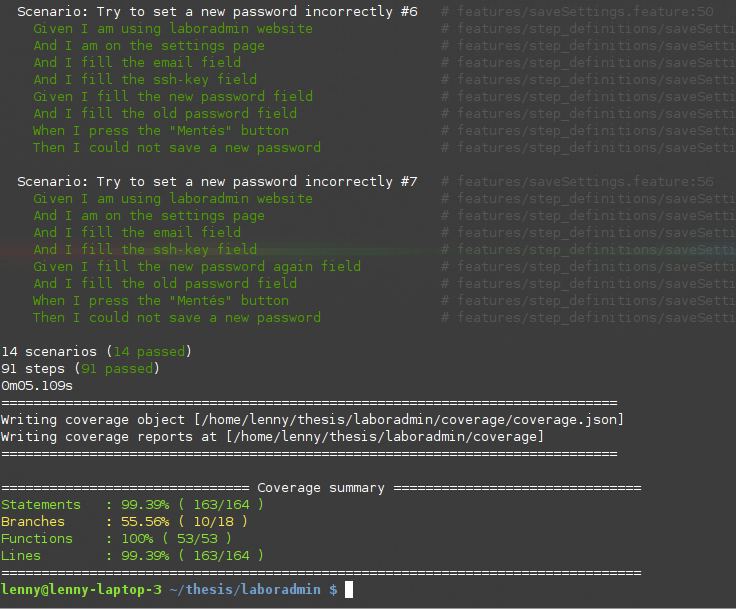
\includegraphics[width=\textwidth]{figures/test-result.png}
	\caption{Part of the Tests' Output}
	\label{fig:test-results}
	\end{figure}

